\documentclass[tizk]{standalone}

\usepackage{fontspec}
\setmainfont{LexendDeca}
\setsansfont{montserrat}
\setmonofont{Cascadia Code PL}

\usepackage[fixed]{fontawesome5}
\usepackage{tikz}
\usetikzlibrary{positioning}
\usetikzlibrary{arrows}
\usetikzlibrary{decorations}
\usetikzlibrary{shapes.symbols}

\begin{document}

\begin{tikzpicture}[
    scale=2,
    ->,>=latex,shorten >=1pt,
    node distance=2.25cm,
    bend angle=15,
    every node/.append style={align=center},
]
    \node (user) {\fontsize{14}{10}\selectfont\faIcon{grin-beam-sweat}};
    \node[draw,fill=white,right=of user] (daemon) {Service réseau\\+\\Parser};
    \node[draw,fill=white,right=of daemon] (crypto) {Module\\cryptographique};
    
    \draw (user) edge[bend left] node[above]{Demande\\de cachet} (daemon);
    \draw (daemon) edge[bend left] node[below]{Cachet} (user);
    
    \draw (daemon) edge[bend left] node[above]{Donnée\\nettoyée} (crypto);
    \draw (crypto) edge[bend left] node[below]{Donnée\\cachetée} (daemon);
    
    \draw (crypto) edge[loop right,distance=1cm] node[draw,fill=white,tape]{Secret} (crypto);
\end{tikzpicture}

\end{document}